\chapter{Introduction}

%%%%%%%%%%%%%%%%%%%%%%%%%%%%%%%%%%%%%%%%%%%%%%%%%%%%%%%%%%%%%%%%%%%%%%
\section{Overview}
\begin{cdrfigure}[Underground detector illustration]{2x5kt-3d}{The LBNE underground liquid argon detector design as of January of 2015. The design consisted of two liquid argon detector module each with 5~kt fiducial volume.}
% 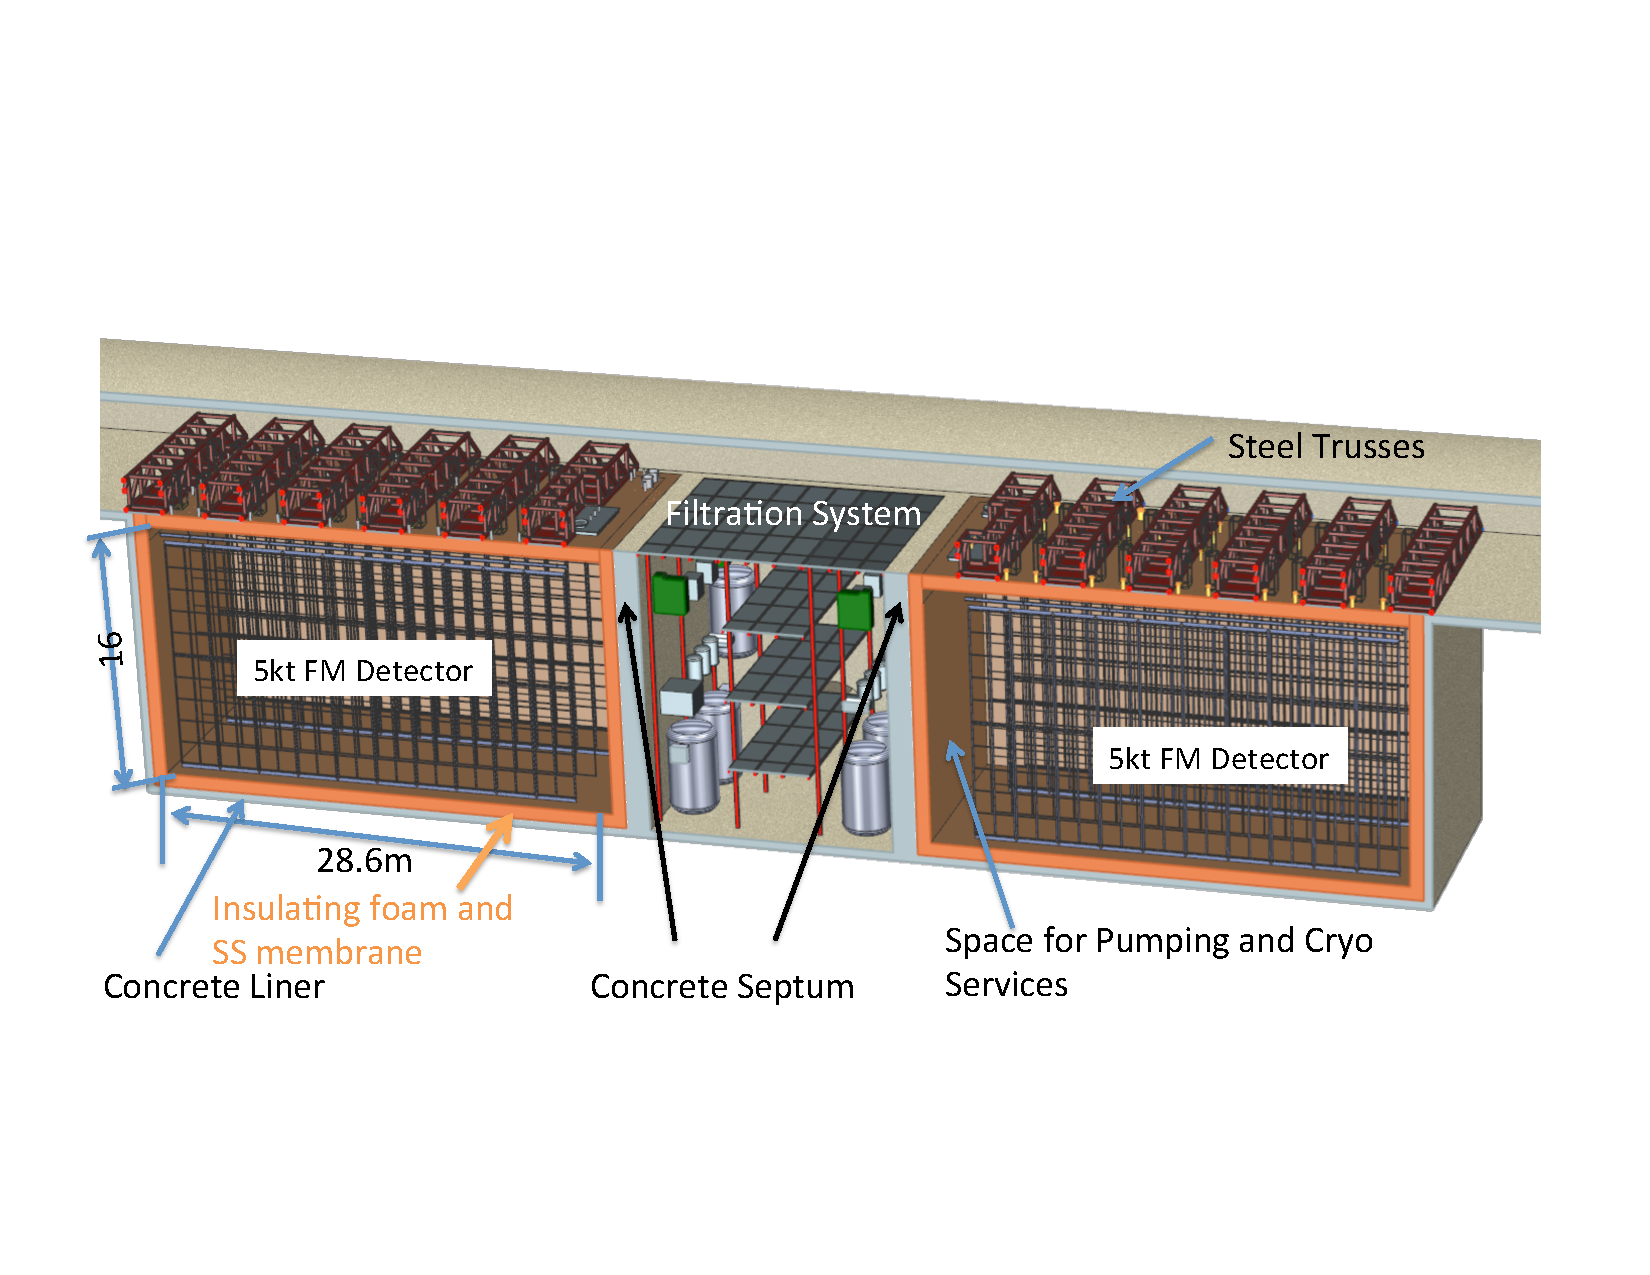
\includegraphics[width=\textwidth]{2x5kt-3D.pdf}
 \end{cdrfigure}
 \fixme{Missing figure in repo}

The former LBNE Far Detector Project team has prepared this design document which describes the single-phase liquid argon time projection chamber (LArTPC) that was being developed for the LBNE experiment. This report reflects the design status of January 2015, which marks the end of the LBNE collaboration and the start of the new DUNE collaboration. As the DUNE collaboration moves forward, it is anticipated that the collaboration will grow and the scope of the experiment will increase. The LBNE detector consisted of two detector modules each with a fiducial volume of 5~kt to be located at the 4850L of the Sanford Underground Research Facility (SURF). Figure~\ref{2x5kt-3d} shows the 3D model of the detector. Throughout this document the detector is referred to as the LAr-FD. 

The LAr-FD is proposed as the starting point for the design of the DUNE single-phase far detector. The full scope of the DUNE experiment consists of four 10-kt detector modules to reach the desired fiducial mass of 40~kt, which would enable a compelling research program in long-baseline and underground neutrino physics and in nucleon decay studies. The ultimate goal in the operation of the facility and experimental program is to measure fundamental physical parameters, explore physics beyond the Standard Model and better elucidate the nature of matter and antimatter. 

The basic components of this detector type are a cryostat to contain the liquid argon (LAr),  a  Time Projection Chamber (TPC) detector mechanism immersed in the LAr to detect charge deposited in the detector, a photon system to register light, a readout electronics system and a cryogenic system to keep the LAr temperature at 89~K and maintain the required purity.  The cryostat and cryogenics systems will be managed by the LBNF project, therefore descriptions of these systems are not included in this document. 

In a single-phase LArTPC, a uniform electric field is created within the TPC volume between cathode planes and anode wire planes. Charged particles passing through the TPC interact with the argon and generate both VUV photon and ionization electrons. The electrons drift in the applied electric field to the anode planes. The anode planes consist of (listed in order from the outside in) four wire planes, a grid plane, two stereo induction planes and a collection plane. The bias voltage to each plane is set so that ionization electrons drift between the grid and the two induction planes, to be collected on the last plane. Readout electronics amplify and continuously digitize the induced waveforms on the sensing wires at 2~MHz, and transmit these data to the data acquisition (DAQ)  system for processing. The wire planes are oriented at different angles allowing a 3D reconstruction of the particle trajectories. In addition to these basic components, a photon-detection system provides a trigger for proton decay and galactic supernova neutrino interactions. 


The design of the LAr-FD has been developed and refined over the past five years. The starting point was the ICARUS  T600 system \cite{Icarus-T600}, and the process was informed and guided by the experience with small  LArTPCs in the U.S., particularly ArgoNeuT~\cite{argoneut-url} and MicroBooNE~\cite{microboone-url}. The LAr-FD concept is designed for assembly from small, independent %elements 
units that can be repeated %almost indefinitely 
as many times as necessary in any dimension to form the entire  assembly within a large cryostat. Each of the units provides an independent mechanical structure to support the elements it contains. 
 The size of the units is defined by the restrictions placed by the local site and logistical issues.  The detector units will be manufactured in advance of the detector installation, so they must be small enough to be shipped and stored using standard transport containers. They must physically fit in the shafts at SURF and %be able to 
 be transported underground. 
 
 The modular design offers several advantages.
The units can be thoroughly  tested prior to installation, reducing installation time. %  and the actual installation can be quickly performed. 
Construction of the major components can be done at multiple sites.
% The design also allows for multiple construction sites for the major components. %The modular design allows one to 
 The design can accommodate a wide range of detector volumes, containing anywhere from a few to several hundred units in a straightforward way, with small and predictable risk. Scaling in other areas of  LArTPC detector technology, namely cryostat construction, LAr purification and electronics readout has been incorporated into the design.



%%%%%%%%%%%%%%%%%%%%%%%%%%%%%%%%%%%%%%%%%%%%%%%%%%%%%%%%%%%%%%%%%%%%%%
\section{LAr-FD Components}
\label{sec:larfd-components}

%%%%%%%%%%%%%%%%%%%%%%%%%%%%%%%%%%%%%%
\subsection{Time Projection Chamber}

The Time Projection Chamber (TPC) is the active detection element of the LAr-FD. The construction concept is  shown schematically in the upper right illustration of Figure~\ref{fig:single-phase-overview}.  A TPC is located inside each cryostat vessel and is completely submerged in LAr at 89~K. Five planes line up across the width: three Cathode Plane Assemblies (CPA)   interleaved with two Anode Plane Assemblies (APA). These planes are oriented vertically and  parallel to the beamline such that the electric fields applied between them are perpendicular to the beamline. Sufficient space is maintained between the detector an the cryostat walls to prevent high voltage discharge. 


\begin{cdrfigure}[Detector Overview Slide for January 2015 configuration]{single-phase-overview}{Left: Illustration of the APA design. 2.3-m by 6-m steel frames form the core of the APAs. Wires are wound about the planes to form the grid plane (not shown), the U and V induction planes and the collection plane. Electronic readout is mounted on one end. The lower APA plane is hung from the top plane to form a 12-m-tall unit. Upper-Right: Schematic showing the orientation of the TPC inside the Cryostat. Lower-Right: The APAs and CPAs are hung from the top of the cryostat using mounting rails. The rails also are used in the installation process to move the planes to the final position. }
 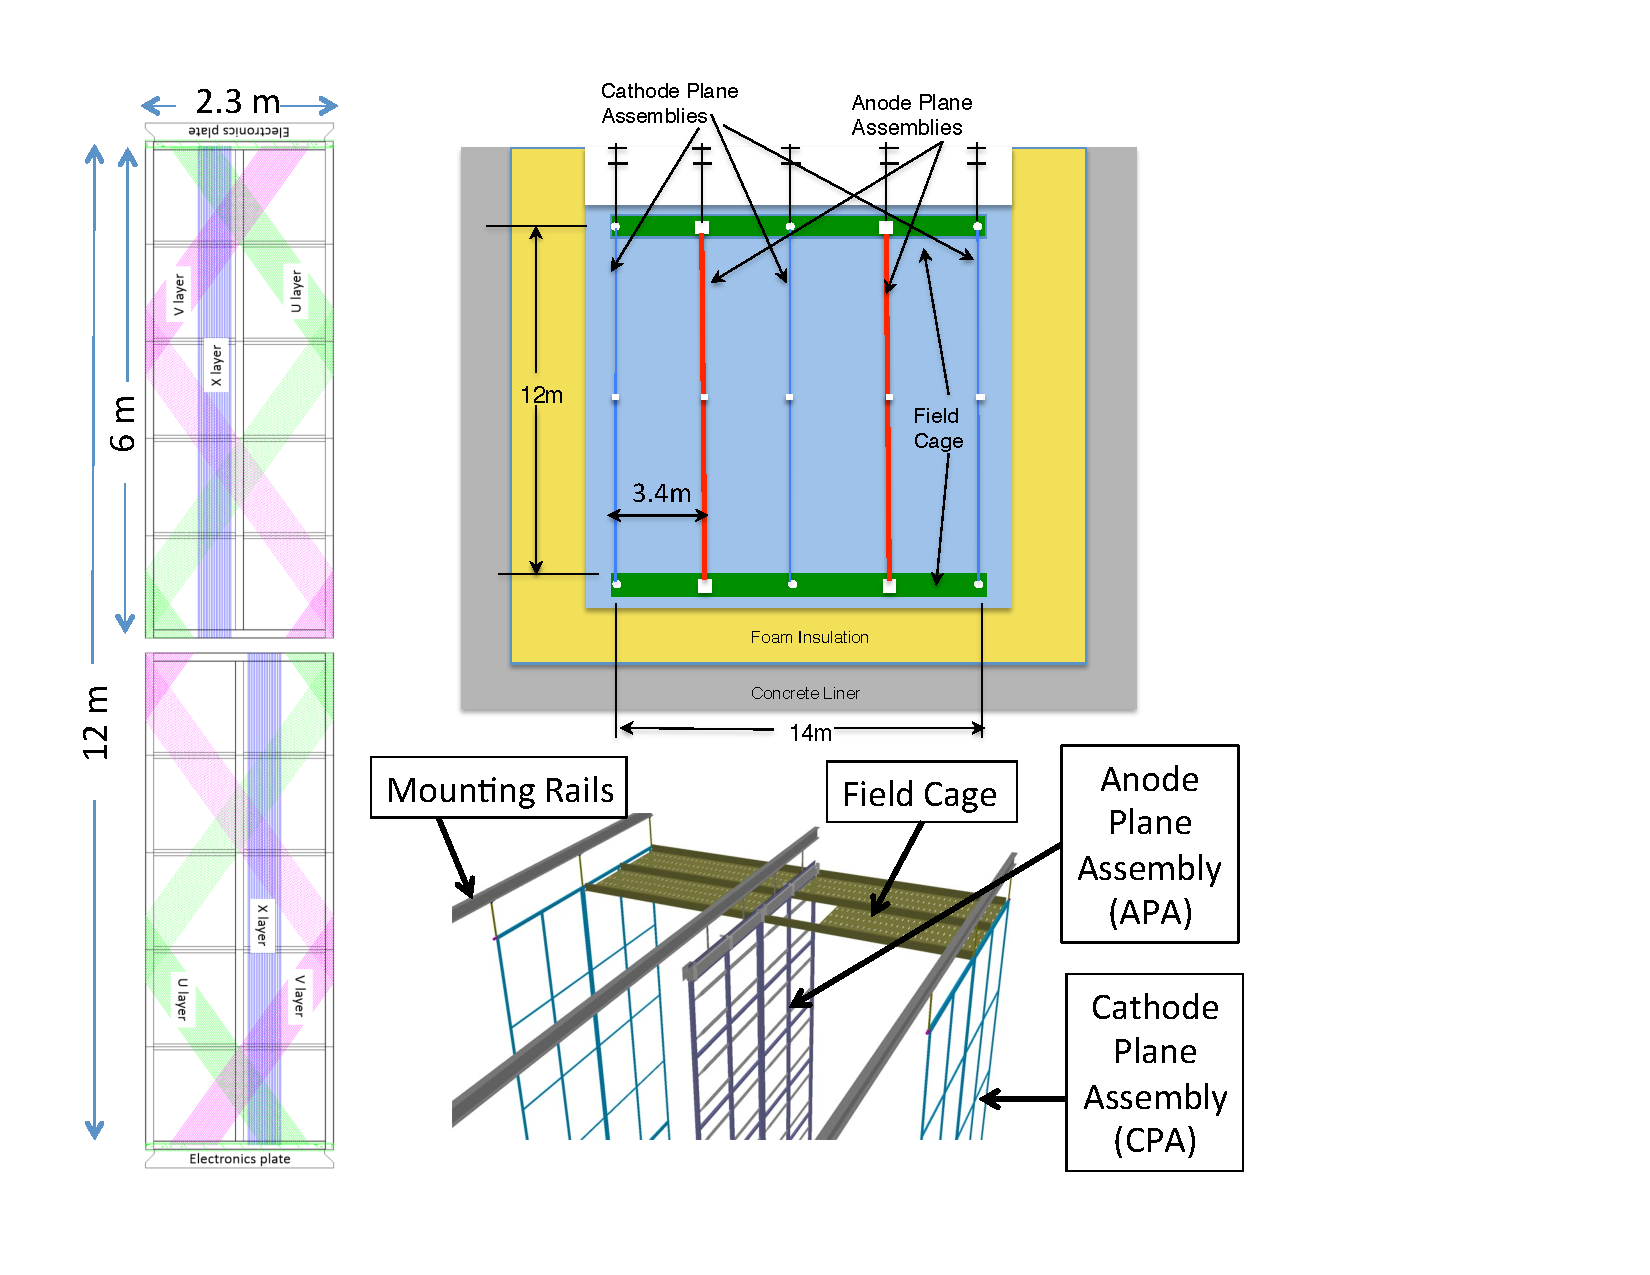
\includegraphics[width=1.0\linewidth]{single-phase-overview.pdf}
\end{cdrfigure}
 
As seen on the left of Figure~\ref{fig:single-phase-overview} the APAs are constructed as 2.3-m-wide, 6-m-tall units. Each APA has three wire planes that are connected to readout electronics; two induction planes (labeled ``U'' and ``V'' in Figure~\ref{fig:single-phase-overview}) and one collection plane (``X''). A fourth wire plane, grid plane (``G''), is held at a bias voltage but is not instrumented with readout electronics. The grid plane improves the signal-to-noise ratio on the U plane and provides electrostatic discharge protection for the readout electronics. The electronic readout is from a single end so that two units can be hung together with minimal gap between the top and bottom units. The APAs are mounted inside the cryostat on rails which run the length of the cryostat (Figure~\ref{fig:single-phase-overview} lower-right). Two rows of wire planes, each two APAs high and 13 deep, instrument each cryostat forming a 30-m-long detector. A total of 52 APA are needed for a 5-kt fiducial volume detector. 

 The CPAs are also manufactured in 2.3-m-wide stainless steel units and are hung from similar mounting rails as the APAs. Insulating G-10 rods connect the CPAs to the rails and provide the needed electrical isolation. Each cryostat  needs 78 CPAs for the three rows.% of CPAs. 
 The maximum electron-drift distance between a CPA and an adjacent APA is 3.4~m. A ``drift cell'' is associated with the volume between any APA and CPA. As seen in Figure~\ref{fig:single-phase-overview}, each of the far detector modules has four drift cells each 3.5~m wide 12~m high and 30~m deep.  A ``field cage'' surrounds the top and ends of the cryostat to ensure uniformity of the electric field. The field cage is assembled from panels of FR-4 sheets with parallel copper strips connected to resistive divider networks.

The size of a liquid argon detector is normally %defined by 
quoted in terms of its mass. However, several metrics are used and need to be clearly defined if comparisons are to be made. The total liquid volume %or 
and mass of a detector module (cryostat) %the detector is 
are defined by the total amount of liquid argon contained;% in the cryostat; 
9.2~kt per cryostat in this case. %for the detector described in this report. 
Space inside the cryostat is needed for the membrane convolutions \fixme{new term to me}, cryogenic services, installation, the volume of the APAs themselves, and an insulation region for HV protection, which is 0.5~m for the LAr-FD. These volumes reduce the total instrumented volume for each %TPC module 
cryostat to 6.9~kt. Finally, in any physics analysis fiducial volume cuts will need to be applied to the data. The cuts will depend on the physics process itself but for the purpose of defining the detector size, the cuts for the oscillation physics are used. These cuts %applied to the detector volume which 
lead to a total fiducial mass of two 5-kt detector modules, as shown in Figure~\ref{fig:10kt-fiducial-mass}. A cut of 10~cm on the upstream end of the detector is applied to ensure that a given event originated inside the detector and not from a muon generated in the rock. A cut of 140~cm downstream of the detector is applied so that muon momentum can be determined by multiple scattering. Finally, a cut of 30~cm on each side of the APAs is applied to ensure that a neutrino interacting in the fiducial volume will be sufficiently contained to have a good energy measurement.

\begin{cdrfigure}[Fiducial mass of 10-kton detector]{10kt-fiducial-mass}{Fiducial mass of 10-kton detector}
 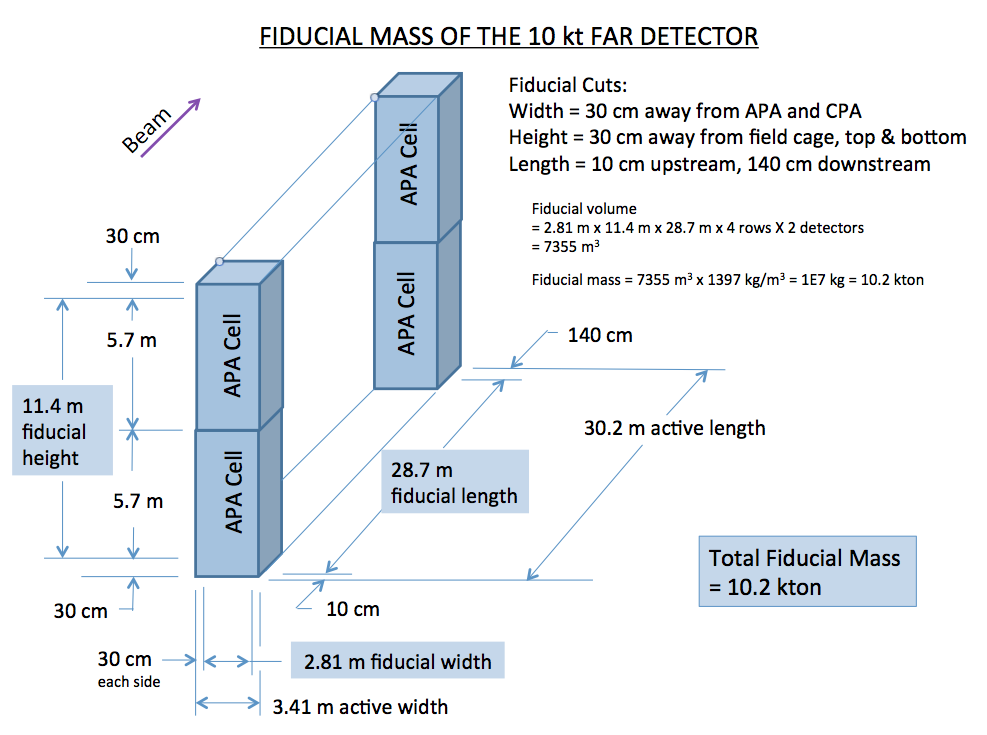
\includegraphics[width=\textwidth]{fiducial-mass-10kt-jan2015.png}
 \end{cdrfigure}

%%%%%%%%%%%%%%%%%%%%%%%%%%%%%%%%%%%%%%
\subsection{Electronics, Readout and Data Acquisition}
\label{sec:det_electronics}


CMOS technology, with a noise minimum at 89~K, permits the front-end electronics to reside in the LAr (henceforth ``cold electronics''), as close to the anode wires as is practical. This minimizes capacitance and therefore signal noise, and benefits LAr purity by not residing in the ullage gas. The cold electronics architecture is comprosed of a front-end shaping/filtering stage (FE ASIC), an analog-to-digital conversion stage (ADC ASIC), and a communication/control stage (digital ASIC). The signal feedthroughs are all located on top of the cryostat, where they are most accessible, are at low hydrostatic pressure, and pose no risk of LAr leakage. The cold electronics multiplex at 1:32, which lowers the cable count to what can be accommodated by the planned number of feedthroughs, and mitigates contamination from cable outgassing by reducing the volume of cables in the ullage gas.

The data acquisition system (DAQ) handles the signals from the LArTPC and photon detection once they are outside the cryostat and packages the data into events within runs for offline analysis.  The logic runs in FPGAs extensively use the Ethernet protocol, which feeds data to commodity computers and network switches  for event building and triggering. This uses a modern software framework that captitalizes on scalable parallelization with multicore machines. The primary data transfer path in the DAQ reads out interactions from neutrinos (beam and atmospheric), proton decay and other underground physics phenomena and cosmic-ray muons with no zero suppression --- these events occur rarely (the most frequent are the cosmic muons at a rate of about one per minute).  A separate data-transfer path works with zero-suppressed data to provide both the triggering for the above events and a continuous readout of all data, which can be filtered for study of low-energy physics phenomena.  These two readout paths are used in combination for supernova events to maximize the information collected, which is dependant on the %investment 
space available for buffering.  The DAQ is partitioned into sections that are more independent than in most HEP experiments; this is done to %allow 
practically eliminate periods of downtime of more than one section of the detector at a time, % to be practically eliminated, 
which is %useful 
important for supernova detection.

%%%%%%%%%%%%%%%%%%%%%%%%%%%%%%%%%%%%%%
\subsection{Photon-Detection System}

Identification of the different possible charged-particle types depends on accurate measurements of ionization along tracks. This requires accurate determination of the time of interaction, or event time, $t_0$, which leads to the absolute location of the event along the drift axis, and allows the determination of $Q_0$,  the 
true ionization charge.

For non-accelerator physics events, $t_0$ is not known a priori. However, LAr is an excellent scintillator, generating of order $10^{4}$ 128-nm photons per MeV of deposited energy.  Detection of scintillation photons provides a prompt signal that allows unambiguous location of particle positions along the drift axis.

The reference design for the photon detection system is based on acrylic bars, which are either coated in TPB or doped in bulk. The 128-nm photons interact with the TPB on the surface and 430-nm light is re-emitted. The signals will be routed out of the cryostat to standard readout electronics.

Twenty light-guide and SiPM assemblies, or ``paddles'', will be installed within each APA frame prior to wire winding. The SiPM signals will be used as a software ``trigger'' in the DAQ to define the event time, t$_0$, for non-accelerator events. This system provides a $t_0$ signal throughout the entire detector in contrast to a system similar to that used in MicroBooNE and ICARUS, where light is detected outside the detector volume. 

%%%%%%%%%%%%%%%%%%%%%%%%%%%%%%%%%%%%%%%%%%%%%%%%%%%%%%%%%%%%%%%%%%%%
\section{Detector Installation and Operation}
\label{sec:det-install}

Detector components will be shipped in sealed containers to the far site by truck and lowered to the cavern. Shipping containers will be moved to a clean area over the septum between the cryostats. There the components will be unpacked from the sealed container and lowered  through an access hatch into the cryostat. 

The construction of the two cryostats and the installation and commissioning activities will be staged such that both TPCs can be tested cold while one cryostat still remains available as a potential LAr storage vessel. The LAr in one cryostat can be transferred to the other, and back again, if necessary, until all the tests complete successfully. Once both TPCs are known to work properly at LAr temperature, the second fill will take place.

To protect the membrane on the floor of the cryostat during TPC installation, a temporary floor will be installed. After each pair of APAs is installed, they will be connected to the DAQ system and the wire integrity will be tested. All wires on previously installed APA pairs will also be tested. The wire integrity test will be performed during cryostat cool-down as well. A relatively slow cool-down rate will ensure that the temperature-induced stresses in the APA frames and wires are kept well below the level experienced during testing. 

An installation and integration detector mock-up will be constructed at Fermilab to confirm that interfaces between detector systems are well defined and to refine the installation procedures. 


%%%%%%%%%%%%%%%%%%%%%%%%%%%%%%%%%%%%%%%%%%%%%%%%%%%%%%%%%%%%%%%

\section{Far Detector Requirements}

The requirements for the far detector TPC can be found in the requirements documentation \cite{lar-fd-req} and are summarized here.  

\subsection{Detector Requirements: Beam Neutrino Physics}

In order to be sensitive to the mass hierarchy, the baseline of the
experiment is required to be in excess of
1000~km~\cite{sci-opp,baselineprd}.  To optimize the simultaneous
constraint on the mass hierarchy and the ability to measure
$\delta_{CP}$, a baseline of 1300~km is needed.

The sensitivity of the experiment scales with the product of the
fiducial mass, the event-detection efficiency, and the acceptance of
the event selection requirements. \fixme{acceptance of ... requirements? I don't get it} The fiducial volume cuts are set so
that events with primary vertices within the fiducial volume are
detected with high efficiency and are contained well enough to
contribute to the oscillation analysis.  The fiducial volume is
assumed to be set at least 1.5~m from the far edges of the active
detector volumes, on the sides of the detectors that the beam exits,
and 30~cm from the boundaries of the active volumes for all other
boundaries, \fixme{from all other `sides'?} which are dominantly defined by the field cages.  The
volume inside the wire planes is to be defined as non-fiducial.
The event timing for beam-induced neutrino scatters
shall be precise enough to correlate the events with the
beam spill times.  % do we want to measure neutrino speed?  We have the longest baseline.

% These requirements are from Table 4.2 in the Scientific Opportunities document

Events will be selected and classified in order to reduce the
backgrounds of the analyses and to focus attention on only those
events with well-modeled efficiency; thus the efficiency for
selecting an analysis-quality event is not expected to be 100\%.  The
event-selection efficiency for $\nu_e$~CC interactions shall be at
least 80\% after selection requirements for incident neutrinos with
energies above 100~MeV.  For $\nu_\mu$~CC interactions, the selection
efficiency shall be at least 85\% for the same range of neutrino
energies.  For neutral current events, a selection efficiency of 90\%
is required.

The determination of the physics outputs requires a very small
systematic uncertainty on the event detection and selection
efficiency, as much of the information is carried by the rates of
$\nu_e$ and $\bar\nu_e$ appearance events and their ratios to the
$\nu_\mu$ and $\bar\nu_\mu$ samples.  The total uncertainty on the
signal yields is required to be less than 1\% from
far-detector-related uncertainties.  For all of these efficiencies, 
fractional systematic uncertainties of less than 0.5\% are required.  These
uncertainties will require the formation of control samples in the
data, therefore events that are not selected as analysis quality still will
need to be detected and counted as such.  %We require that 
A neutrino
interaction of any sort with its vertex in the fiducial volume,
depositing above 50~MeV of ionization energy in the detector is required to be
detected by charge signals on the wires in the TPC, even if they are
not selected by the analysis cuts.  %We require that 
The systematic
uncertainty on the fiducial mass of the detector, the product of the
fiducial volume and the density of the liquid argon, %to 
is required to be less than
0.5\%.  Because the fiducial volume cuts are applied to the primary
vertex location, the resolution on the primary vertex is thus required
to be better than 25~mm.

The background rates for $\nu_e$-CC and $\nu_\mu$-CC events are required
to be no more than half of the relevant signal rates, and the relative
systematic uncertainties on the predictions of the background rates 
are required to be no larger than 5\%.  The misidentification
rate of neutral-current neutrino scatters as $\nu_e$-CC events is
required to be less than 1\%.  The misidentification rate of
$\nu_\mu$-CC events as $\nu_e$-CC events is required to be less than
1\%.  For $\nu_\mu$ disappearance studies, the misidentification rate
of neutral-current neutrino scatters as $\nu_\mu$-CC events is
required to be less than 1\%.

As more data are collected, the shapes of the distributions of the
reconstructed neutrino energies become increasingly important in
reducing the uncertainties in the measured parameters.  The event-by-event resolution on the reconstructed neutrino
energy for $\nu_e$-CC events %is 
shall be no wider than 15\%/$\sqrt{E({\rm GeV})}$,
 and for $\nu_\mu$-CC, no wider than 20\%/$\sqrt{E({\rm GeV})}$.  
The resolution of the reconstructed neutrino energy in
neutral-current interactions is required to be no wider than
30\%/$\sqrt{E({\rm GeV})}$ for neutrinos with energies between 200~MeV
and 6~GeV.  The energy resolution on stopping hadrons (protons and kaons) is required
to be 1-3\% based on the measured ionization and range.

The average neutrino energy-scale calibration is required
to be better than 5\% for both $\nu_e$-CC and $\nu_\mu$-CC
events~\cite{docdb8741}.  % it's 1-2% in the sci-opp book
The calibration of the energy resolution function is required to be better than ??\%
for both electron and muon events (``needs study'').

\subsection{Detector Requirements: Supernova Burst Neutrino Physics}

In order to perform measurements of supernova-burst neutrinos, %we require that 
the detection efficiency (including hardware and analysis
selection effects) for a single 5-MeV electron is required to be in excess of 90\%
averaged over the active volume of the detector, and that %the detection efficiency 
for the scintillation light flash from a 10-MeV
electron to be in excess of 50\% averaged over the active volume of the
detector.  The energy resolution of electron tracks in SNB neutrino
events is required to be better than 15\% in the range 5-100~MeV in
order to study the properties of SNB neutrino spectra.  The cosmic-ray
and radiological background to low-energy $\nu_e$-CC events shall be low enough to measure
a supernova burst within the Milky Way.

The far detector is required to be able to collect data continuously,
in order to maximize the acceptance of atmospheric neutrino scatters,
SNB events, and nucleon decays.  The data-acquisition system is
required to be able to buffer at least two minutes of continuous, 
untriggered data for long-term storage in order to preserve a detailed
record of a supernova burst.  These data are to be collected with minimal impact
from zero suppression, either with a lower threshold, or a generous amount of samples
in both time and space near triggered signals. The detector, data-acquisition system, and
online processing shall be able to trigger a supernova-burst event and
provide a prompt alert. The absolute time of arrival of SNB
neutrino events is required to be known to 0.1~ms.  The relative time
difference between any two SNB events is also required to be known to
0.1~ms.  The angular resolution on supernova-burst neutrinos shall be
sufficient to point them to a common location in the sky.  Prompt de-excitation
gammas produced in association with low-energy charged-current interactions
shall be identified and separated from radiological backgrounds and electronics noise.

\subsection{Detector Requirements: Atmospheric Neutrino Physics}

The detection efficiency for neutrino interactions is required to be
independent of energy, angle, and arrival time, for events with
primary vertices within the fiducial volume.  The cosmic-ray backgrounds
for atmospheric neutrino physics shall be small enough so as not to impact
the analysis's sensitivity significantly.  The more stringent requirements
on cosmic-ray backgrounds for proton decay will suffice for the atmospheric
neutrino analyses, which are less sensitive to backgrounds.

\subsection{Detector Requirements: Nucleon Decay Physics}

The separation of charged kaons from protons, pions, and muons shall be unambiguous
and accomplished
via $dE/dx$ vs. residual range measurements, as well as interactions at the
ends of the tracks.  The cosmic-ray background shall be low enough to achieve the
proton decay science objective.  

\subsection{Derived Detector Performance Requirements}

The detection efficiency for a minimum-ionizing particle (MIP)
traveling close to the CPA is required to exceed 99\%.  The
signal-to-noise ratio for a MIP traveling close to the CPA is thus
required to be 9:1 or better, in all three detection planes,
regardless of the orientation of the track.

The detector uptime shall be greater than 90\% during beam running.
At least part of the detector shall be operational at all times.

The uncertainty on the electron loss due to the finite electron
lifetime shall be known to better than 1\%.  This requirement can be
satisified with a high electron lifetime, a stable electron lifetime,
and regular monitoring with purity monitors and {\it in situ}
measurements.

Electromagnetic showers shall be identified by their topology.  The
energy resolution on individual EM showers is required to be
3\%/$\sqrt{E({\rm GeV})}$.  The muon momentum resolution is required
to be better than 5\% for fully-contained muon tracks, and better than
15\% for partially-contained muon tracks.

The misidentification rate of photons from $\pi^0$ as electrons is
required to be less than 2\% from measuring the $dE/dx$ in the
beginning of the electromagnetic shower, coupled with reconstructed
event topological information, such as the identification of second
electromagnetic showers and the displacement of the shower start from
the primary vertex.

Single-track events shall be separated from multi-track events with a
high efficiency.  Protons, pions, and kaons recoiling from 
charged-current interactions with kinetic energies above
21~MeV~\cite{argoneut_proton_spectra} shall be counted and
identified.  This requirement is coupled to similar requirements on the near detector,
where a closer match between identification efficiencies of each final state in the far
and the near detector provides better cancellation of systematic uncertainty.
Energy deposits from neutrons
originating in neutrino scatters shall be recorded.

The far detector shall communicate the data to the LBNE global DAQ,
which shall record the data on long-term storage media easily
accessible to the collaboration.

The detector shall retain its resolution on $dE/dx$ up to $15\times
$MIP, in order to separate heavily-ionizing particles from one
another, and to measure overlapping particles.

Reconstruction ambiguities arising from wrapped wires shall not
degrade the pattern-recognition abilities of the far detector and its
software such that the above requirements are not met.  In order for
each event to be reconstructible without ambiguity, each
induction-plane wire may intersect any collection-plane wire at most
once.  More ambiguity may result in charge deposits reconstructed far
away from their true locations, worsening the particle counting,
energy, and particle identification performances.

Studies have shown that the separation of electrons from photons
using the ionization density of the first portion of an electromagnetic shower
depends most critically on the first 2.5~cm of the shower.  That, and the need
to identify low-energy electrons, protons, and pions gives a wire pitch
requirement of no more than 5~mm.

The electric field shall be sufficiently uniform and the detector alignment
sufficiently stable and well known in order for the muon momentum measurement
from multiple scattering requirement to be met.

\subsection{Engineering Requirements}

In order to reduce the cosmogenic backgrounds for SNB, nucleon decay,
atmospheric neutrinos and beam neutrinos, the detector is to be situated
at the 4850~ft level of the SURF facility. \fixme{The prev sounds like a physics req} The far detector underground hall shall
accommodate the construction of a class 100,000 clean room for detector
construction. \fixme{say why clean env needed; LAr purity issues?}  Concrete floors shall be sealed in %areas of 
clean room environments
and in the high bay of the cavern.  Showers are to be provided for workers underground
to remove dust and debris.  A solid waste disposal station consisting of a pad
large enough to accommodate two 4'$\times$6' dumpsters shall be provided near
the surface support buildings.

There shall be control rooms both on the surface and underground, with monitoring
of detector parameters and data flow.  Adequate electrical power, water, air,
cryogenics support, and networking shall be provided via the shafts.   In case
one shaft becomes inoperable, the other shaft is required to provide egress, ingress,
and sufficient services to ensure the safety of the staff and equipment.
Sufficient airflow is required to reduce buildup of radioactive radon gas.

\fixme{More requirements -- safety? TJ?}

%%%%%%%%%%%%%%%%%%%%%%%%%%%%%%%%%%%%%%%%%%%%%%%%%%%%%%%%%%%%%%%
\section{Principal Parameters}

The principal parameters of the LAr-FD are given in Table~\ref{tab:param-summ-larfd}. 
\fixme{This is for the closeout LBNE design -- 10-kt detector is 5+5?}
\begin{cdrtable}[LAr-FD Principal Parameters for 10-kt Detector]{lp{7cm}}{param-summ-larfd}
{LAr-FD Principal Parameters for 10-kton Detector}
Parameter & Value \\ \toprowrule
Active (Fiducial) Mass &   13.8 (10.2)~kton \\
\colhline
Number of Detector Modules (Cryostats) &  2 \\
\colhline
Drift Cell Configuration within Module &  2~wide $\times$ 2~high $\times$ 13~long \\
\colhline
Drift Cell Dimensions  &  2 $\times$ 3.4~m wide (drift) $\times$ 6~m high $\times$ 2.3~m long \\
\colhline
Detector Module Dimensions &  14~m wide $\times$ 12~m high $\times$  30~m long \\
\colhline
Anode Wire Spacing &  $\sim$4.8~mm \\
\colhline
Wire Planes (Orientation from vertical) & Grid (0$^\circ$), Induction 1 (36$^\circ$), Induction 2 (-36$^\circ$), Collection (0$^\circ$) \\
\colhline
Drift Electric Field &  500~V/cm \\ 
\colhline
Maximum Drift Time & 2.1~ms \\
\end{cdrtable}
%%%%%%%%%%%%%%%%%%%%%%%%%%%%%%%%%%%%%%%%%%%%%%%%%%%%%%%%%%%%%%%%
\section{Design Considerations}

TPCs operated to date have been constructed with an anode wire spacing
in the range of 3~mm (ICARUS) to 4.8~mm (Fermilab cosmic-ray
stand). The amount of ionization charge collected on the wires
increases with larger wire spacing, resulting in a better
signal-to-noise ratio without serious consequences (the radiation
length of LAr is $\sim$~30 times larger than the typical wire
spacing). The electron-$\pi^0$ separation efficiency of a TPC with
5-mm wire spacing is only a few percent lower than one with 3-mm wire
spacing. It is also clear that a TPC with larger wire spacing requires
fewer wires and readout channels, resulting in lower cost.  As the
wire spacing becomes larger, however, spatial resolution degrades in
the plane parallel to the wires, while resolution remains good in the
remaining axis pointing along the electric field as that axis is
digitized in time samples.  This difference in resolutions along the
three axes, if too big, will lead to anisotropy in efficiencies,
resolutions, and particle ID performance.  The 5-mm wire spacing is
expected to be adequate for discerning short stubs from supernova
neutrino scattering elecrons which should create signals in
approximately ten adjacent wires for a 10-MeV electron.  Counting
short protons near the interaction vertex requires good resolution for
short tracks.  Furthermore, ambiguities in associating features between
planes become easier to break when the spatial resolution is better.%
\fixme{could put this later. TJ?}

If hits can be unambiguously reconstructed and associated between
planes, then only two wire planes are required to reconstruct events
in three dimensions.  However, three wire planes are needed in order
to break ambiguities and provide $N+1$ redundancy.  In many events,
one or more tracks will travel parallel or nearly parallel to the
wires in one or more of the planes, reducing one plane's contribution
to the spatial resolution.  The other two planes' hits will be able to
reconstruct these tracks in three dimensions.  Furthermore, the
wrapping of the induction-plane wires introduces a discrete ambiguity
in interpreting the hits on these wires.  Hits that arrive on
different wires at similar times, because they come from portions of
tracks and clusters that are similar distances from the anode plane,
create ambiguity in the association of hits between planes.  The
wrapping allows for more combinations, as tracks and clusters from
either side of the APA can contribute to the signals on any induction
wire.

The collection-plane wires are oriented vertically ($0^\circ$) in
order to minimize both the wire length and the electronics noise,
as well as to provide readout on the ends of the APA frames for
each wire.  These wires do not wrap around the APA frames and so
they provide unambiguous two-dimensional information about the
event.  Calorimetry is most commonly performed using the
collection-plane wires, therefore low noise is important, though
induction-plane wires provide additional measurements of the same
drifting charge.

% cite LBNE-docdb-9374 -- wire angle change request, 8981 and 9886,
% the tech board meeting documents -- trade study

A study of wire orientation~\cite{docdb2836} was performed that uses
the sum of the numbers of wires a photon from $\pi^0$ decay traverses
in all three planes before it converts.  This figure of merit is
designed to optimize topological separation of neutral-current events
from charged-current electron neutrino scatters.  In this study, the
optimum orientation of the induction plane wires should be between
$\pm40^\circ$ and $\pm60^\circ$ when the collection plane wires are at
$0^\circ$ for beam neutrino physics. The ideal orientation for the
more isotropic low-energy events, e.g., supernova-neutrino
interactions, is $\pm60^\circ$.  Selecting induction-plane wire angles
in this range necessitates wrapping the wires around the sides of the
APA frames so that readout electronics can be located on the top or
bottom of the TPC.  As a result, it is natural to arrange the APA's
vertically in a two-high configuration.

Wrapping the induction-plane wires however creates pattern-recognition
difficulties arising from the discrete ambiguity of which segment of
the wire contributed any given signal.  If the wires wrap around more
than once, so that a particular induction-plane wire intersects a
particular collection-plane wire more than once, then the ambiguity is%%%%% Anne to here 4/6 5pm
unresolvable with two readout planes and a third one is required, with
a slightly different angle so as to to create repeated solutions of
three wires intersecting.  Even with the proposed 44.3$^\circ$ and
45.7$^\circ$ solution of the initial design, however, ambiguities
resurface when multiple hits arrive on different wires at similar
times.  Misassociating hits between views can have the consequence of
displacing the three-dimensional reconstructed location of the charge
deposit by the vertical distance required to wrap an induction-plane
wire around once, or approximately five meters in the CD-1 design.
Even with the most sophisticated reconstruction algorithms, it is
expected that even a small fraction of misassigned hits will create
difficulties in energy reconstruction, track identification, and
particle ID which may be difficult to simulate to the accuracy
required by the physics program.

In order to reduce the impact of hit assignment ambiguity on
reconstruction, an angle of $\pm35.71^\circ$ was chosen for the
induction-plane wires~\cite{docdb-9374,docdb8981,docdb9886}.  The APA
design with this angle improves on the CD-1 design in a number of
ways.  The length of the APA is shorter at 6~meters, allowing it to be
stiffer using the same materials.  The 2.3-meter APA width was chosen
to facilitate construction and allow standard, over-the-road
transport. The wire angle is such that no induction-plane wire
intersects any given collection-plane wire more than once,
significantly reducing the categories of events for which combinations
of hits can be misassigned.  The exact wire angle and APA dimensions
were further constrained by the desire to have an integer multiple of
128 readout channels per APA so as to efficiencly assign channels to
front-end boards.  In this design, the collection-plane wires are 6~m
long and the induction-plane wires are 7.3~m long.

The choice of cryostat width is based on the desired cryostat shape
and cavern span. From a cryogenics standpoint, the ideal cryostat for
a modular TPC would be a cube since membrane-cryostat capital and
operating costs scale linearly with the surface area. This shape is
not ideal for cavern excavation, however. In the absence of a
geotechnical investigation for the cavern location, the cavern span
has been limited to $\sim$30~m on the advice of rock engineers. A
detector width of 14~m results after making allowance for cryostat
insulation, and personnel access both above and within the cryostat.

A drift field of 500~V/cm was chosen based on experience from similar
detectors such as ICARUS, ArgoNeuT and the Fermilab cosmic-ray test
stand. At this electric field, $\sim$ 30\% of the ionization electrons
produced by the passage of a minimum ionizing particle (MIP) recombine
and create scintillation light that provides a fast trigger. The
remaining ionization electrons drift to the APA and produce wire-plane
signals. The TPC could function at higher or lower drift fields but
the relative yields of scintillation light and ionization electrons
would change. The use of a higher drift field would require more care
in the design of the high-voltage systems. The electron drift velocity
is 1.6~mm/$\mu$s at 500~V/cm.

The 14~m width of the the detector can be divided into four drift
cells with a maximum drift length of 3.41~m each. This drift cell
length was chosen based on experience from other detectors, the
required minimum signal-to-noise ratio and high-voltage
considerations. The required minimum signal-to-noise ratio of 9:1
ensures that the tracking efficiency will be 100\% throughout the
entire drift cell. The TPC must be capable of detecting the smallest
signal (1~MeV) produced in interactions that LBNE will study. This
situation occurs when a MIP travels parallel to a wire plane and
perpendicular to the orientation of the wires in the plane. A MIP
loses 2.1~MeV of energy in each cm of travel, producing $\sim$ 40,000
ionization electrons along every 5~mm section of the track. About
28,000 electrons escape recombination and, ignoring the effects of LAr
purity and diffusion, would all drift to one collection plane
wire. The capacitance due to the maximum-length 7.3~m wire is 164~pF
resulting in an equivalent noise charge (ENC) of 500 electrons in the
CMOS amplifiers. The signal-to-noise ratio would therefore be 53:1 if
all of the ionization electrons arrived at the wire. For a maximum
drift distance of 3.41~m and a drift field of 500~V/cm, the required
voltage on the cathode plane is 173~kV. This is within the range of
commercially available high-voltage cables and within the range of
current designs for cryogenic feedthroughs. Additional R\&D would be
needed for longer maximum drift lengths.

Ionization electrons will be lost due to impurities in the LAr. The
fraction that survive passage to the anode planes is $e^{t/\tau}$,
where$t$ is the drift time and $\tau$ is the drift-electron
lifetime. The maximum drift time is the maximum drift length divided
by 1.6~mm/$\mu$s which equals 2.3~ms for LBNE. The ICARUS detector has
achieved a drift electron lifetime of 6 -- 7~ms. The Materials Test
Stand (described in Section~\ref{sec:mts}) regularly achieves a
drift-electron lifetime of 8 -- 10 ms. The Fermilab Liquid Argon
Purity Demonstrator achieved a liftime of $>$ 3~ms during initial
tests. Based on this experience, and by careful selection of materials
in the ullage, a drift-electron lifetime at least as good as ICARUS is
expected. The signal-to-noise ratio would be 36:1 for a drift electron
lifetime of 6~ms. A minimum lifetime of 1.4~ms is required to meet the
9:1 signal-to-noise ratio requirement.

The cloud of drifting ionization electrons will spread out in space
due to the effects of diffusion. The maximum transverse $RMS$ width of
the electron cloud is 2.4~mm for the chosen drift distance and drift
field. This is well matched to the 5~mm wire spacing.


\nomenclature{ADC}{analog-to-digital converter}
\nomenclature{APA}{anode plane assembly}
\nomenclature{APD}{avalanche photodiodes}
\nomenclature{ArgoNeuT}{Mini LArTPC Exposure to Fermilab's NuMI Beam}
\nomenclature{ASIC}{application-specific integrated circuit}
\nomenclature{BGR}{band-gap reference}
\nomenclature{CAD}{computer-aided design}  
\nomenclature{CDF}{one of two decommissioned collider detectors at Fermilab's Tevatron, along with D-Zero}  
\nomenclature{CF}{conventional facilities} 
\nomenclature{CFD}{computerized fluid dynamics} 
\nomenclature{CPA}{cathode plane assembly}
\nomenclature{DAQ}{data acquisition}
\nomenclature{DCM}{data concentrator module}
\nomenclature{DC}{direct current}
\nomenclature{DCM}{Data concentrator modules}
\nomenclature{D-Zero}{one of two decommissioned collider detectors at Fermilab's Tevatron, along with CDF}
\nomenclature{EM}{electromagnetic}
\nomenclature{ENC}{equivalent noise charge}
\nomenclature{ESH}{Environment, Safety and Health}
\nomenclature{FEM}{front-end module}
\nomenclature{FESHM}{Fermilab's ES\&H Manual}
\nomenclature{FFT}{Fast Fourier Transform}
\nomenclature{FIRUS}{Fire and Utilities; Fermilab site-wide, high-reliability, remote monitoring system used to monitor building fire panels and various utilities throughout the lab}
\nomenclature{FLARE}{Fermilab Liquid Argon Experiments}
\nomenclature{FPGA}{field-programmable gate array}
\nomenclature{FR-4}{flame resistant 4}
\nomenclature{FSE}{field-shaping electrode}
\nomenclature{GAr}{gaseous argon}
\nomenclature{GLACIER}{NASA's General Laboratory Active Cryogenic International Space Station Experiment Refrigerator}
\nomenclature{LNGS}{Gran Sasso National Laboratory}
\nomenclature{G10/FR4}{a fire rated electrical-grade dielectric made with and epoxy material reinforced with a woven fiberglass mat}
\nomenclature{GTT}{Gaztransport \& Technigaz}
\nomenclature{HSSD}{High Sensitivity Smoke Detection}
\nomenclature{HV}{high voltage}
\nomenclature{HVAC}{heating, ventilation and air conditioning}
\nomenclature{ICARUS}{Imaging Cosmic and Rare Underground Signals, experiment at the LNGS}
\nomenclature{INFN}{Istituto Nazionale della Fiscia Nucleare} 
\nomenclature{IHI}{Ishikawajima-Harima Heavy Industries}
\nomenclature{IT}{integration prototype}
\nomenclature{IU}{Indiana University}
\nomenclature{LANNDD}{Liquid Argon Neutrino and Nucleon Decay Detector}
\nomenclature{LAPD}{Liquid Argon Purity Demonstrator}
\nomenclature{LAr}{liquid argon}
\nomenclature{LAr1}{one-kiloton LAr prototype for LBNE's LAr-FD}
\nomenclature{LAr-FD}{LBNE's Liquid Argon Far Detector}
\nomenclature{LArSoft}{a reconstruction software package for LAr detectors}
\nomenclature{LArTPC}{liquid argon time projection chamber}
 \nomenclature{LBNE}{Long-Baseline Neutrino Experiment}
\nomenclature{LED}{light-emitting diode}
\nomenclature{LEM}{large electron multiplier}
\nomenclature{LEMO}{a push-pull connector made by the LEMO company in Switzerland}
\nomenclature{LHe}{liquid helium}
\nomenclature{LN}{liquid nitrogen, also written LN$_2$ and LN2}
\nomenclature{LNG}{liquefied natural gas}
\nomenclature{LOTO}{lockout/tagout; an OSHA safety practice }
\nomenclature{LPG}{liquefied petroleum gas}
\nomenclature{LVDS}{low-voltage differential signaling}
\nomenclature{MCT}{membrane cryostat test}
\nomenclature{MicroBooNE}{A 100-ton LArTPC located along Fermilab's Booster neutrino beamline }
\nomenclature{MINERvA}{A neutrino-scattering experiment that uses the NuMI beamline at Fermilab}
\nomenclature{MINOS}{Main Injector Neutrino Oscillation Search, a Fermilab experiment}
\nomenclature{MIP}{minimum ionizing particle}
\nomenclature{MIT}{Massachusetts Institute of Technology}
\nomenclature{MOS}{metal-oxide semiconductor}
\nomenclature{MOSFET}{metal-oxide-semiconductor field-effect transistor}
\nomenclature{MTU}{master timing unit}
\nomenclature{MUX}{multiplex}
\nomenclature{Bis-MSB}{1,4-bis[2-(2-methylphenyl)ethenyl]-benzene, a wavelength-shifting chemical}
\nomenclature{MTS}{Materials Test Stand}
\nomenclature{N or N2}{nitrogen}
\nomenclature{NASA}{National Aeronautics and Space Administration}
\nomenclature{NBTI}{negative bias temperature instability}
\nomenclature{NC}{neutral current}
\nomenclature{NICADD}{Northern Illinois Center for Accelerator and Detector Development NOvA}
\nomenclature{NIM}{Nuclear Instruments and Methods (journal)}
\nomenclature{NIST}{National Institute of Standards and Technology}
\nomenclature{NIST}{National Institute of Standards and Technology}
\nomenclature{NSF}{National Science Foundation}
\nomenclature{NOvA}{NuMI Off-Axis Neutrino Appearance experiment at Fermilab}
\nomenclature{OD}{outer diameter}
\nomenclature{ODH}{oxygen deficiency hazard}
\nomenclature{OPERA}{Oscillation Project with Emulsion-Racking Apparatus, at CERN and LNGS}
\nomenclature{OSHA}{Occupational Safety and Health Administration}
\nomenclature{PC}{personal computer}
\nomenclature{PC-4}{Fermilab building, Proton Center building number 4}
\nomenclature{PCI}{peripheral component interconnect}
\nomenclature{PDA}{photon detection assembly}
\nomenclature{PDE}{photon-detection efficiency}
\nomenclature{PE}{photo-electron}
\nomenclature{PLC}{programmable logic controller}
\nomenclature{PMT}{photomultiplier tube}
\nomenclature{PPE}{personnel protective equipment}
\nomenclature{PRV}{pressure-relief valve}
\nomenclature{QC}{quality control}
\nomenclature{RC}{resistive capacitive}
\nomenclature{ROOT}{An object oriented framework for large-scale data analysis developed at CERN}
\nomenclature{SCR}{silicon controlled rectifier}
\nomenclature{SDSTA}{South Dakota Science and Technology Authority}
\nomenclature{SIMOPS}{simultaneous operations study}
\nomenclature{SiPM}{Silicon photomultiplier}
\nomenclature{SM}{stress-migration}
\nomenclature{S/N}{signal-to-noise }
\nomenclature{SS}{stainless steel}
\nomenclature{TC}{thermal cycling}
\nomenclature{TDDB}{time-dependent dielectric breakdown}
\nomenclature{TDU}{timing distribution unit}
\nomenclature{TPB}{tetraphenyl butadiene, a wavelength shifting chemical}
\nomenclature{TPC}{Time Projection Chamber}
\nomenclature{USB}{universal serial bus}
\nomenclature{UV}{ultraviolet}
\nomenclature{VME}{a computer bus standard}
\nomenclature{VUV}{vacuum ultraviolet light}
\nomenclature{WARP}{Wimp Argon Program}
\nomenclature{WBS}{Work Breakdown Structure}
\nomenclature{WLS}{wavelength shifter}

\nomenclature{A}{ampere (also mA, kA)   }
\nomenclature{atm}{atmosphere}
\nomenclature{bar}{bar (also mbar, etc.)}
\nomenclature{barg}{bar gauge (deprecated per Wikipedia)}
\nomenclature{b}{barn, a measure of cross section; bit (also Mb, Gb, etc.)}
\nomenclature{B}{byte (also MB, GB, etc.)}
\nomenclature{Bq}{becquerel}
\nomenclature{C}{coulomb}
\nomenclature{cf}{cubic foot (also ft$^3$)}
\nomenclature{cfm}{cubic feet per meter (also ft$^3$/m)}
\nomenclature{Ci}{curie}
\nomenclature{eV}{electron-volt (also keV, MeV, GeV) }
\nomenclature{F}{farad (also pF, nF )}
\nomenclature{ft}{foot or feet }
\nomenclature{gal}{gallon}
\nomenclature{gpm}{gallons per minute (also gal/min)} 
\nomenclature{G}{gauss (also mG) or gradient (in magnets)}
\nomenclature{g}{gram (also mg, kg)}
\nomenclature{Hz}{hertz (s-1)}
\nomenclature{h}{hour}
\nomenclature{in}{inch }
\nomenclature{K}{kelvin} 
\nomenclature{l}{liter}
\nomenclature{m}{meter (also nm, micron, mm, cm, km) }
\nomenclature{min}{minute }
\nomenclature{MICA}{type of dielectric material used in capacitors}
\nomenclature{MS}{mega samples}
\nomenclature{N}{newton}
\nomenclature{NPO}{type of dielectric material used in capacitors}
\nomenclature{QFP}{quad flat pack}
\nomenclature{R}{roentgen}
\nomenclature{Pa}{pascal}
\nomenclature{psi}{pounds per square inch}
\nomenclature{rad}{radian (also mrad) }
\nomenclature{s}{second (also ns, $\mu$s, ms) }
\nomenclature{scfm}{standard cubic foot per minute }
\nomenclature{SHV}{safe high voltage, a type of HV cable connector}
\nomenclature{t}{ton}
\nomenclature{T}{Tesla}
\nomenclature{V}{volt (also mV, kV, MV)}
\nomenclature{VA}{volt-ampere (also mVA, kVA, MVA)}
\nomenclature{VAC}{Volts alternating current (also mVAC, kVAC)}
\nomenclature{VUV}{vacuum ultraviolet}
\nomenclature{W}{watt (also mW, kW, MW) }
\nomenclature{yd}{yard }
